\subsection{Fixed-Node Diffusion Monte Carlo (FN-DMC)}
Diffusion Monte Carlo is a projector method that evolves a trial wavefunction with a Hamiltonian in imaginary time and projects out the ground-state wavefunction.  For practical simulations of fermions, the fixed-node approximation is introduced, which depends only on set of electronic positions where a trial wave functions is equal to zero.  This approximation is different than approximations typically used in quantum chemistry calculations, and in this work we demonstrate that we can generate high quality nodal surfaces for full electron-ion wave functions. 

In the limiting case that  the trial wavefunction has the same nodal surface as the exact ground-state wavefunction, the final ground-state energy will be exact. Approximate nodal surface can be generated through optimization of the full wave function. Such approximate nodal surfaces have been tested and validated on a wide range of systems, and consistently provide an excellent approximation of the exact ground-state energy,  comparable to the state of the art in \textit{ab initio} simulations [{\bf refs.~here}]. In addition the energies generated with FN-DMC are variational with regards to the ground state energy.

%With advances in wave function optimization, 
In all but a handful of previous QMC simulations,  ions are "clamped" to their equilibrium positions. Such an assumption is not fundamentally required by FN-DMC.  It is possible to optimize thousands of wave function parameters simultaneously with variational Monte Carlo ~\cite{Nightingale_Linear,Umrigar_Linear,Brown_Bench} .   In our previous work we found that the most important effect to optimize for were the nodes due to electron-electron correlations~\cite{Tubman_ECG}, and in this regard we use more sophisticated electronic terms in the wave function than the ion part of the wave function.

\subsection{Electron Wavefunction and Optimization}
The are several different approaches for generating high quality wave functions ~\cite{Umrigar_Alleviation,Toulouse_Bench, Brown_Bench,Seth_Bench}. We use an initial guess for the wavefunction that is generated from complete active space self-consistent field (CASSCF) \cite{Chaban_MCSCF,Szabo} calculation using the quantum chemistry package GAMESS \cite{GAMESS}. The optimized orbitals are then used in a second order configuration interaction (SOCI) calculation to generate a series of configuration state functions (CSF)~\cite{Clark_Bench}. The multi-CSF expansion of the wavefunction  can be expressed in the following form,
\begin{align}
\Psi_{SOCI}(\vec{r})=\sum\limits_{i=1}^{N_{CSF}}\alpha_i\phi_i(\vec{r}), \label{eq:psi_gms}
\end{align}
where $\vec{r}$ refers to the spacial coordinates of all the electrons. $\phi_i(\vec{r})$ are the CSF generated from SOCI. We used the cc-pV5Z basis for all the atomic systems and Roos Augmented Triple Zeta ANO basis for molecular systems~\cite{dunning,roos}. We then impose cusp condition on each molecular orbital~\cite{cusp} and add a Jastrow factor to the wave function to include electron correlation~\cite{Kato}. Our Jastrow factor contains one, two and three body terms. The full wave function being optimized is then
\begin{align}
\Psi_e(\vec{r})=e^{J(\vec{r},\vec{\beta})}\sum\limits_{i=1}^{N_{CSF}}\alpha_i\phi_i(\vec{r})\label{eq:psie}
\end{align}
We optimized the CSF and Jastrow coefficients $\vec{\alpha},\vec{\beta}$ simultaneously with QMCPACK \cite{QMCPACK}.

\subsection{Electron-Ion Wavefunction}

\begin{figure}[t]
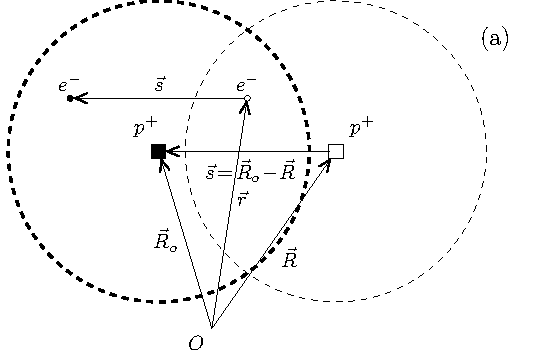
\includegraphics[width=9cm]{fig1a.pdf}
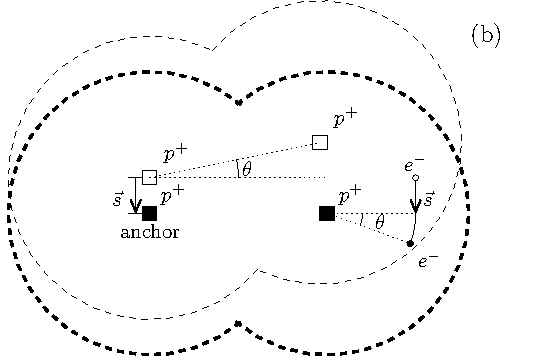
\includegraphics[width=9cm]{fig1b.pdf}
\caption{Dragged node approximation: {\bf (a)} For hydrogen atom, we assume the entire wavefunction shifts with the ion. This process can be visualized by following a contour of the wavefunction. The thick dashed circle represents a contour of the electron wavefunction when the proton is at its reference position $\vec{R}_o$ and the thin dashed circle represents the same contour when the proton has moved to a new position $\vec{R}$. To evaluate the ion-dependent electron wavefunction $\bar{\psi}_e(\vec{r},\vec{R})$, we simply map the electron to its proper place in the reference wavefunction $\psi_e(\vec{r})$. That is, $\bar{\psi}_e(\vec{r},\vec{R})=\bar{\psi}_e(\vec{r}+\vec{s},\vec{R}_o)=\psi_e(\vec{r}+\vec{s})$ where $\vec{s}$ is the shift required to put the proton back to its reference position. {\bf (b)} For H$_2^+$, we pick one of the protons as an "anchor" and approximate the new wavefunction by dragging the reference wavefunction with the "anchor" proton. We also rotate the wavefunction to align its axis of symmetry with the orientation of the two protons. \label{fig:drag}}
\end{figure}

Once a satisfactory electronic wave function has been obtained, we construct the electron-ion wave function using the ansatz we previously investigated~\cite{Tubman_ECG},
\begin{align}
\Psi_{ei}(\vec{r},\vec{R})=\psi_I(\vec{R})\bar{\psi}_e(\vec{r},\vec{R}), \label{eq:psi}
\end{align}
where $\vec{R}$ includes spatial coordinates of all ions. The ion wave function consists of simple products of Gaussian wave functions over each nuclei pair,
\begin{align}
\psi_I(\vec{R})\propto \prod\limits_{i,i<j}e^{-a(\vert \vec{R}-\vec{R}_j\vert-b_{ij})^2},
\label{wfs_ions}
\end{align}
where $a$ is a contraction coefficient for the ion wave function that we optimize for each system and $b_{ij}$ are taken to be the equilibrium distances between the nuclei at the minimum of the potential energy surface of the clamped nuclei. In Fig.~\ref{fig:drag} we demonstrate this strategy for the simple cases of a hydrogen atom and a H$_2^+$ molecular ion. Although the dragged-node technique is developed with atomic and diatomic systems in mind, it is not difficult to generalize it for use in larger systems or even apply to parts of a bigger system, e.g., treating light ions as quantum particles and heavy ions as "clamped". 